\documentclass[a4paper]{article}

\usepackage[spanish]{babel}
\usepackage{graphicx}
\usepackage{amsmath, amssymb}
\usepackage[margin=2cm]{geometry}
\usepackage{fancyhdr}
\usepackage{enumerate}
\usepackage[shortlabels]{enumitem}
\usepackage{parskip}
\usepackage[most]{tcolorbox}
\usepackage[hidelinks]{hyperref}
\usepackage{float}
\usepackage{setspace}
\usepackage{xspace}


\usepackage{tabularx}
\usepackage{ragged2e}
\newcolumntype{L}{>{\RaggedRight\arraybackslash}X}
\newcolumntype{C}{>{\Centering\arraybackslash}X}

% cabecera
\pagestyle{fancy}
\fancyhead[l]{Daniel Soto}
\fancyhead[c]{Problemas de Astronomía \#13}
\fancyhead[r]{\today}
\fancyfoot[c]{\thepage}
\renewcommand{\headrulewidth}{0.2pt} % linea horizontal

%% Definicion de comandos para formato de unidades fisicas %%
\newcommand{\m}{\text{m}}
\newcommand{\cm}{\text{cm}}
\newcommand{\mm}{\text{mm}}
\newcommand{\km}{\text{km}}
\newcommand{\s}{\text{s}}
\newcommand{\N}{\text{N}}
\newcommand{\g}{\text{g}}
\newcommand{\kg}{\text{kg}}
\newcommand{\Msolar}{\text{M}_\odot}
\newcommand{\Mterrestre}{\text{M}_\oplus}
\newcommand{\AU}{\text{AU}}
\newcommand{\ly}{\text{ly}}
\newcommand{\nT}{\text{nT}}
\newcommand{\keV}{\text{keV}}
\newcommand{\MeV}{\text{MeV}}
\newcommand{\GeV}{\text{GeV}}
\newcommand{\atoms}{\text{atoms}}
\newcommand{\K}{\text{K}}
\newcommand{\J}{\text{J}}
\newcommand{\particles}{\text{particles}}
\newcommand{\protones}{\text{p}^+}
\newcommand{\electrones}{\text{e}^-}
\newcommand{\Gy}{\text{Gy}}
\newcommand{\My}{\text{My}}
\newcommand{\nm}{\text{nm}}
\newcommand{\blank}{\rule{2cm}{0.4pt}\xspace}
\newcommand{\mol}{\text{mol}}



\newcounter{problema}

\newtcolorbox[use counter=problema]{problema}[1][]{%
	breakable,
    colback=gray!15,
    colframe=gray!60,
    fonttitle=\bfseries,
    title={Problema~\theproblema:},
    boxrule=0.5mm,
    arc=3mm,
    boxsep=5pt,
    left=8pt,
    right=8pt,
    top=6pt,
    bottom=6pt,
    #1
}


\begin{document}

\begin{problema}

Después de que un meteorito golpea la superficie de un planeta, los fragmentos de escombros siguen trayectorias parabólicas a medida que vuelven a caer a la superficie. Cuando el impactador LCROSS golpeó la Luna, los escombros formaron una columna de material que alcanzó una altura de 10 kilómetros y regresó a la superficie alrededor del cráter.

    \begin{figure}[H]
        \centering
        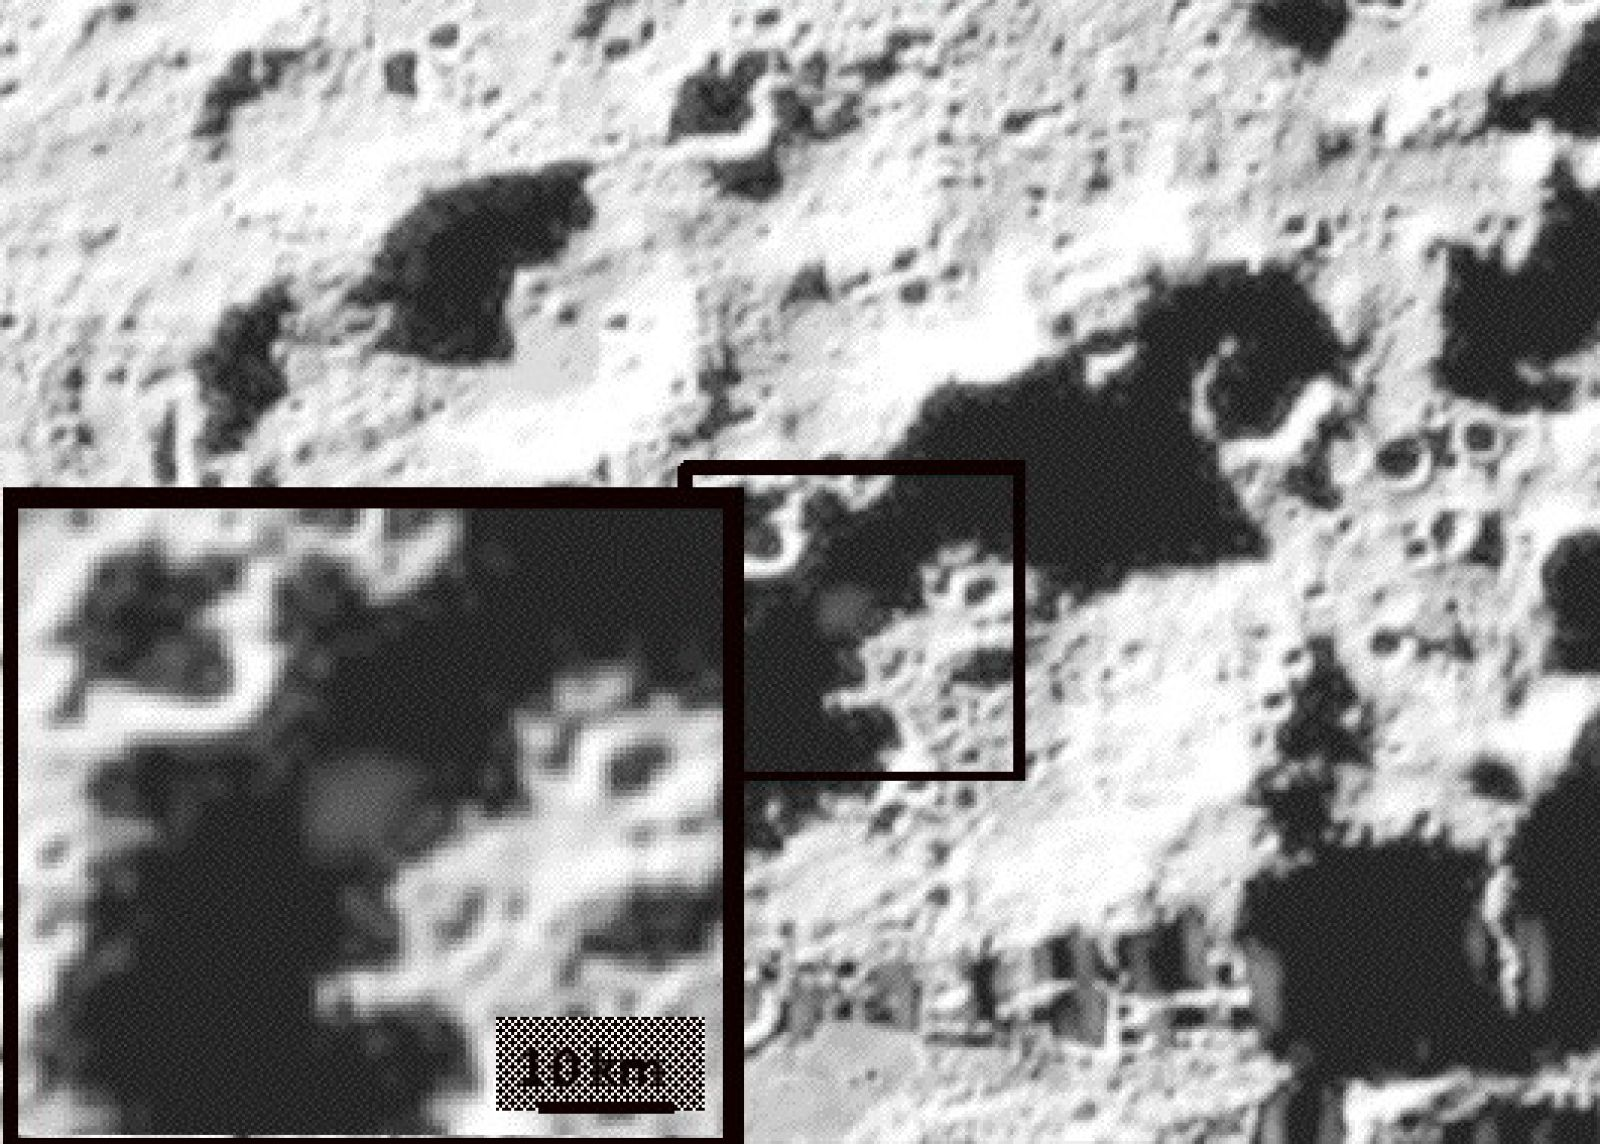
\includegraphics[width=0.7\textwidth]{LCROSS.jpg}
        \caption{Penacho de escombros del LCROSS visto en la sombra oscura de un cráter lunar. (NASA/LRO)}
        \label{LCROSS}
    \end{figure}

El tamaño del campo de escombros que rodea el cráter puede estimarse resolviendo una ecuación cuadrática para determinar las propiedades de la trayectoria promedio de los escombros. La ecuación que aproxima la trayectoria promedio de las partículas está dada por:

$$
H(x) = x - \frac{g}{2v^2}x^2
$$
\begin{enumerate}
	\item La ecuación da la altura, $H(x)$ en metros, de una partícula promedio eyectada a una distancia $x$ del lugar del impacto, donde $v$ es la velocidad de las partículas en metros/segundo y $g$ es la aceleración de la gravedad en la superficie de la Luna en $\m/\s^2$. Factoriza esta ecuación para encontrar sus dos 'raíces', que representan la distancia inicial de eyección desde el centro del cráter de impacto y la distancia final de aterrizaje de las partículas desde el centro del cráter.

	\item ¿A qué distancia del centro del cráter alcanzaron los escombros su altitud máxima?

	\item ¿Cuál fue la altitud máxima de los escombros a lo largo de su trayectoria?

	\item Resuelve esta ecuación parabólica para el caso específico de la eyección de LCROSS, donde $v = 200 \m/\s$ y $g = 2 \m/\s^2$, para determinar:
	\begin{enumerate}
		\item El radio máximo del campo de escombros alrededor del cráter
		\item La altura máxima de la columna de escombros.
	\end{enumerate}
\end{enumerate}

\end{problema}
[5.2.1]

\begin{problema}

Se producen nubes de escombros cuando un proyectil de alta velocidad impacta una luna o un asteroide. La imagen a la izquierda fue tomada por la nave espacial \textit{Deep Impact} segundos después de que su impactador de $370 \kg$ golpeara el núcleo del Cometa Tempel-1 en 2005.

    \begin{figure}[H]
        \centering
        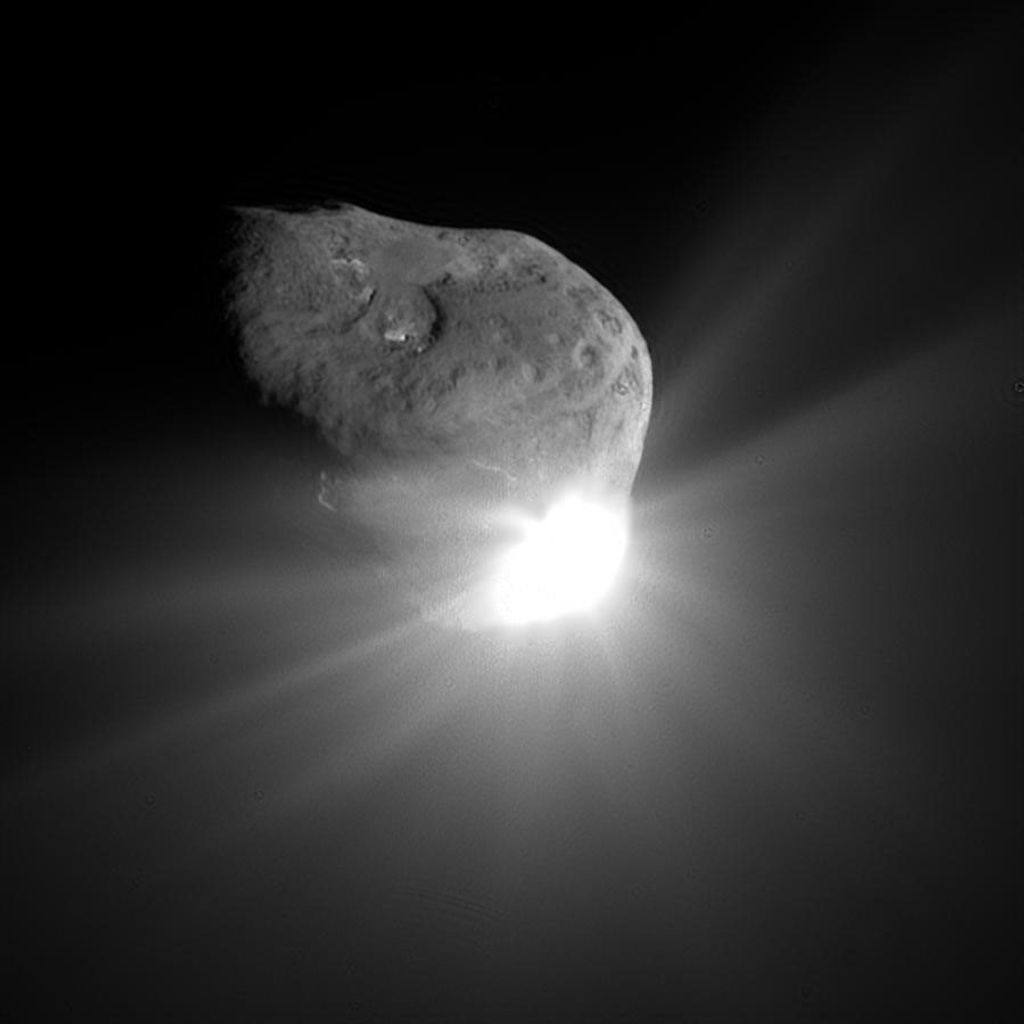
\includegraphics[width=0.7\textwidth]{Tempel.jpg}
        \caption{Penacho de escombros del impacto de \textit{Deep Impact} en el Cometa Tempel-1 (NASA/Deep Impact).}
        \label{Tempel1}
    \end{figure}

Una vez en el pico de su trayectoria, algunas de las partículas de escombros caen de nuevo a la superficie. Su altura sobre la superficie, $H(t)$, viene dada por la función:

$$
H(t) = h_0 - \frac{1}{2}gt^2
$$

donde $h_0$ es su altitud inicial sobre la superficie en metros, y $g$ es la aceleración de la gravedad en $\m/\s^2$.

\vspace{5mm}

\begin{enumerate}
    \item El 9 de octubre de 2009, el impactador LCROSS se estrelló contra la superficie de la Luna con una energía equivalente a unas 2 toneladas de TNT, y produjo un cráter de 350 metros de diámetro. Se observó que el penacho de eyección, que contenía una mezcla de roca lunar calentada y agua atrapada, alcanzó una altura de 10 kilómetros. Si la aceleración de la gravedad en la superficie lunar es $1.6\ \mathrm{m}/\mathrm{s}^2$, ¿cuánto tiempo tardaron las partículas más altas del penacho en volver a caer a la superficie lunar?

    \item El 4 de julio de 2005, la nave espacial \textit{Deep Impact} sobrevoló el Cometa Tempel-1 y lanzó un impactador de $370\ \mathrm{kg}$ que golpeó la superficie del cometa a una velocidad de $10\ \mathrm{km}/\mathrm{s}$, con una energía equivalente a unas 5 toneladas de TNT. Se observó un brillante penacho de eyección, compuesto por una mezcla de partículas de polvo y hielo de agua. Aunque la mayoría de las partículas de escombros fueron expulsadas completamente durante el impacto, algunas partículas de movimiento más lento quedaron atrás y finalmente cayeron de nuevo a la superficie del cometa. Si la altitud máxima de las partículas de escombros que regresaban fue de unos 300 metros, ¿cuánto tiempo tardaron en alcanzar la superficie si la aceleración de la gravedad en este pequeño cuerpo era de solo $0.34\ \mathrm{m}/\mathrm{s}^2$?
\end{enumerate}

\end{problema}
[5.3.3]

\begin{problema}

Durante más de 100 años, los astrónomos han investigado cómo el polvo interestelar absorbe y refleja la luz de las estrellas. Demasiado polvo hace que las estrellas se desvanezcan y se vuelvan invisibles para los telescopios ópticos.

Los observatorios infrarrojos de la NASA, como WISE y Spitzer, estudian los granos de polvo directamente mediante la radiación infrarroja de "calor" que emiten. La cantidad de radiación térmica depende de la composición química de los granos de polvo y de su reflectividad (llamada albedo). A través de estudios detallados del espectro electromagnético de los granos de polvo, los astrónomos pueden determinar su composición química.

    \begin{figure}[H]
        \centering
        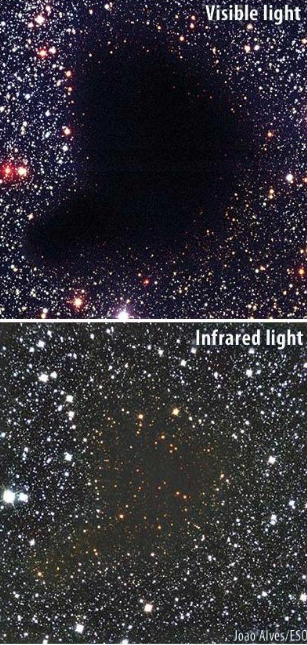
\includegraphics[width=0.5\textwidth]{B68.png}
        \caption{Comparación óptica e infrarroja de la nube de polvo Barnard 68. Arriba: visible (opaca). Abajo: infrarrojo (casi transparente). (ESA/VLT)}
        \label{B68}
    \end{figure}

Las dos imágenes arriba, tomadas con el Very Large Telescope de la Agencia Espacial Europea, muestran la apariencia en el óptico (arriba) y en el infrarrojo (abajo) de la nube de polvo interestelar Barnard 68. Muestran cómo se comportan los granos de polvo en diferentes longitudes de onda. En longitudes de onda visibles, hacen que la nube sea completamente opaca, por lo que las estrellas de fondo distantes no se ven en absoluto. En longitudes de onda infrarrojas, los granos de polvo absorben mucha menos luz infrarroja y la nube es casi transparente.

$$A(m) = c \frac{\left|\frac{m^2-1}{m^2+2}\right|^2}{\mathfrak{I}\left(\frac{1-m^2}{m^2+2}\right)}
$$

La ecuación anterior es un modelo matemático del albedo de un grano de polvo, $A(m)$, en función de su índice de refracción, $m$, que es un número complejo de la forma $m = a - b i$. El denominador $\mathfrak{I}(\ldots)$ es la "parte imaginaria" de la cantidad compleja indicada entre paréntesis. A partir de tus conocimientos sobre números complejos y su álgebra, responde las preguntas siguientes.
\begin{enumerate}
	\item Un astrónomo utiliza una composición de grano de polvo de grafito puro para la cual $m = 3 - i$. ¿Cuál es el albedo de un grano de polvo de $0.1$ micrones de diámetro a:
	\begin{enumerate}
		\item Longitudes de onda ultravioleta de 0.3 micrones ($c = 10.0$)
		\item A una longitud de onda infrarroja de 1 micrón ($c = 0.1$)
	\end{enumerate}
\end{enumerate}
\end{problema}
[5.4.1]



\cite{algebra2}
\bibliographystyle{plainurl}
\bibliography{bibliografia} % Nombre del .bib

\end{document}
